% Leak Trace: technical paper. Build: xelatex leak-trace-paper.tex (twice)
\documentclass[10pt,a4paper]{article}
\usepackage[a4paper,left=24mm,right=24mm,top=24mm,bottom=26mm,headsep=8mm,footskip=11mm]{geometry}
\usepackage{fontspec}
\usepackage{unicode-math}
\setmainfont{TeX Gyre Pagella}[Ligatures=TeX]
\setsansfont{Inter}[Scale=MatchLowercase,BoldFont={Inter SemiBold},RawFeature={-calt}]
\newfontfamily\interbold{Inter Bold}[Scale=MatchLowercase,RawFeature={-calt}]
\newfontfamily\intermedium{Inter Medium}[Scale=MatchLowercase]
\setmonofont{DejaVu Sans Mono}[Scale=0.84]
\setmathfont{Latin Modern Math}
\setmathfont[range=up/{Latin,latin,num}]{texgyrepagella-regular.otf}
\setmathfont[range=it/{Latin,latin}]{texgyrepagella-italic.otf}
\newfontfamily\rupeefont{FreeSerif}
\newcommand{\rs}{{\rupeefont ₹}}
\usepackage{microtype}
\usepackage[english]{babel}
\usepackage{csquotes}
\usepackage{xcolor}
\definecolor{pen}{HTML}{1E2FC6}
\definecolor{form}{HTML}{BF1E58}
\definecolor{ink2}{HTML}{52514E}
\definecolor{rule}{HTML}{E1E0D9}
\definecolor{wash}{HTML}{F3F4FD}
\usepackage{graphicx}
\usepackage{booktabs,tabularx,multirow,array}
\usepackage{amsmath,amsthm}
\usepackage{enumitem}
\setlist{itemsep=2pt,topsep=4pt,leftmargin=1.4em}
\usepackage[font={small,sf},labelfont={bf,color=pen},labelsep=period,justification=raggedright,singlelinecheck=false,skip=6pt]{caption}
\usepackage{titlesec}
\titleformat{\section}{\sffamily\bfseries\large\color{pen}}{\thesection}{0.8em}{}
\titleformat{\subsection}{\sffamily\bfseries\normalsize}{\thesubsection}{0.7em}{}
\titleformat{\paragraph}[runin]{\sffamily\bfseries\small}{}{}{}[.]
\titlespacing*{\section}{0pt}{16pt}{6pt}
\titlespacing*{\subsection}{0pt}{11pt}{4pt}
\titlespacing*{\paragraph}{0pt}{6pt}{0.6em}
\usepackage{fancyhdr}
\pagestyle{fancy}
\fancyhf{}
\renewcommand{\headrulewidth}{0pt}
\fancyhead[L]{\sffamily\scriptsize\color{ink2}Leak Trace · technical paper}
\fancyhead[R]{\sffamily\scriptsize\color{ink2}Seva First Innovation Challenge 2026 · South Zone · Theme 4 · Track A}
\fancyfoot[C]{\sffamily\scriptsize\color{ink2}\thepage}
\fancypagestyle{first}{\fancyhf{}\fancyfoot[C]{\sffamily\scriptsize\color{ink2}\thepage}}
\usepackage{tikz}
\usetikzlibrary{positioning,arrows.meta,calc,fit,backgrounds}
\usepackage[hidelinks]{hyperref}
\usepackage{xurl}
\hypersetup{colorlinks=true,linkcolor=pen,citecolor=pen,urlcolor=pen,pdftitle={Leak Trace: tracing partial, retyped exam-paper leaks to the college that printed them},pdfauthor={Team Leak Trace, Sreyas Institute of Engineering and Technology, Hyderabad},pdfsubject={Seva First Innovation Challenge 2026, South Zone, Theme 4, Track A},pdfkeywords={exam paper leak, fingerprinting codes, traitor tracing, likelihood ratio, anytime-valid inference}}
\usepackage[numbers,sort&compress]{natbib}
\setlength{\bibsep}{2pt}
\renewcommand{\bibfont}{\small}
\usepackage{algorithm}
\usepackage{algpseudocode}
\usepackage{float}
\usepackage{placeins}
\newtheorem{proposition}{Proposition}
\newtheorem{corollary}{Corollary}
\theoremstyle{remark}
\newtheorem*{remark}{Remark}
\setlength{\parskip}{3pt}
\linespread{1.06}
\newcommand{\pr}{\mathbb{P}}
\newcommand{\E}{\mathbb{E}}
\newcommand{\tablefont}{\sffamily\footnotesize}
\newcolumntype{Y}{>{\raggedright\arraybackslash}X}
\newcolumntype{R}{>{\raggedleft\arraybackslash}X}

\begin{document}
\thispagestyle{first}

\begin{flushleft}
{\sffamily\scriptsize\color{form}\MakeUppercase{Technical paper \quad·\quad Seva First Innovation Challenge 2026 \quad·\quad South Zone \quad·\quad Theme 4, Shikshit \& Kaushal Bharat \quad·\quad Track A}}\\[10pt]
{\interbold\fontsize{23}{27}\selectfont\color{pen} Leak Trace: tracing partial, retyped exam-paper leaks to the college that printed them}\\[9pt]
{\sffamily\normalsize Team Leak Trace \quad·\quad Sreyas Institute of Engineering and Technology, Hyderabad}\\[2pt]
{\sffamily\small\color{ink2} Version 1.0, 30 October 2026 \quad·\quad Live demo, code and data: see Appendix~\ref{app:repro}}
\end{flushleft}
\vspace{4pt}
\noindent{\color{pen}\rule{\linewidth}{1.2pt}}

\noindent\begin{minipage}{\linewidth}
\small
\textsf{\textbf{Abstract.}} When an exam paper leaks from one of the hundreds of colleges that print it, the leak usually reaches students as a handful of retyped or photographed questions, and the QR codes, serial numbers and watermarks that exam bodies print do not survive. Leak Trace gives every college a content-identical paper whose arrangement encodes a college-specific codeword in three layers: the order of interchangeable questions, labels and options; faculty-approved wordings; and, new in this paper, \emph{load-bearing marks}, the values in numerical questions and the letter under which each right option sits, which a leaker cannot change without making the leaked answers wrong. A likelihood-ratio decoder reads a leak in any form (typed text, a photographed page read by OCR, or a bare answer key) and names a college only when the evidence makes it at least $T=10{,}000$ times likelier than every other college and $T$ times the number of colleges likelier than a copy from outside the system; otherwise it returns a ranked shortlist. We prove that, under our model of copies made outside the system, the chance that such a copy clears the single-college naming bar is at most $1/T$ (and $2/T$ with the separate two-college test), and that the bound holds at every moment while the lines of a leak are read one by one, so investigators may re-run the decoder as more screenshots surface. In simulations with 500 colleges, seven numbered questions name the source 92\% of the time; across 135{,}000 honest and 148{,}000 adversarial leaks the decoder named an innocent college once, for a copy made outside the system; a leaked answer key with 14 correct answers is named every time; with 16 approved value sets per question, six reworded and shuffled numerical questions are named in 83\% of leaks; and no innocent college was named in 171{,}000 such leaks. A custody design (2-of-3 secret sharing, a codebook derived from the key and a signed Merkle root sent to every principal) means no single official can frame a college or swap a paper undetected. All evaluation so far is synthetic; we state the limits and the pilot that comes next.
\end{minipage}

\vspace{2pt}
\noindent{\color{rule}\rule{\linewidth}{0.6pt}}

\section{Introduction}

Exam papers in India leak often, and when they do, the source is found late or never. Media reports counted 89 suspected paper leaks in the ten years to 2024, 68 of them in state exams; at least 48 papers had to be re-tested, in exams taken by at least 6.5 crore candidates~\citep{newslaundry2024}. NEET-UG 2026 was cancelled nine days after it was held~\citep{moneylife2026}. Universities that affiliate hundreds of colleges have moved from sealed packets to password-protected PDFs that each college prints shortly before the exam: Kannur University does this for its 120 colleges~\citep{southfirst2025kannur}, Bangalore University moved its B.Ed.\ papers to principals' logins with a one-time password 30 minutes before the exam~\citep{etv2025bu}, VTU sends papers online 30 minutes ahead~\citep{udayavani2018vtu}, and JNTU Hyderabad lists \enquote{Electronic Distribution of Examination Papers} among its exam-branch practices~\citep{jntuh2019aqar}. That printing step is where several recent leaks began. On 2 April 2025 a principal-in-charge in Kasaragod received the Kannur PIN at 9:00 and posted four to five of the actual questions to a students' WhatsApp group at 9:04, an hour before the exam~\citep{onmanorama2025b}.

Leaks rarely show a whole page. Karnataka State Law University's Contract Law-I paper was sold in January 2025 as \enquote{two, five, or 10 questions}~\citep{dh2025kslu}. The QR codes, serial numbers and hidden codes that boards now print~\citep{tribune2023haryana,dh2024wbbse,sakshi2025tsssc,nios2026} stay behind on the paper. Sources are therefore found by luck or by police work: Kannur's leak surfaced because an exam squad caught a student copying~\citep{onmanorama2025b}; at Telangana's agricultural university the Vice-Chancellor noticed unusually high marks and CCTV showed a student finishing in ten minutes~\citep{siasat2026pjtsau}; the law-university leak needed phone-to-phone forensics~\citep{dh2025kslu}. Even the NEET-UG 2026 leak, spotted quickly because 45 of 108 chemistry questions matched a circulating \enquote{guess paper} word for word and 90 of 204 biology questions also matched~\citep{theweek2026neet}, took the CBI until August to attribute, with the help of handwriting examination, to three NTA subject experts~\citep{tribune2026cbi}.

While the source is unknown, every college is a suspect and every student who wrote the paper risks a re-exam. Once Kannur's source was known, its sub-committee recommended a re-exam for that one college; the Vice-Chancellor said \enquote{it is not right for everyone to suffer for the mistake of one principal}~\citep{onmanorama2025b}. A fast, specific and calibrated lead would let a university re-examine one college instead of a hundred, clear honest colleges quickly, and give investigators a place to start within minutes. It would also deter: an insider who knows a leak points back to their own college has a strong reason not to leak.


\begin{figure}[t]
\centering
\begin{tikzpicture}[
  font=\sffamily\scriptsize,
  box/.style={draw=pen!70, line width=0.6pt, rounded corners=2pt, fill=wash, align=left, text width=2.55cm, minimum height=1.25cm, inner sep=4pt},
  end/.style={box, fill=pen, text=white, draw=pen},
  arr/.style={-{Stealth[length=4pt]}, line width=0.7pt, draw=pen!80},
  lab/.style={font=\sffamily\bfseries\scriptsize, text=form, anchor=west}]
\node[lab] at (-0.1, 1.05) {BEFORE THE EXAM};
\node[box] (a1) at (1.25, 0) {\textbf{Setter} writes one paper and approves wordings, value sets and movable questions};
\node[box, right=0.42cm of a1] (a2) {\textbf{Two of three officials} combine key shares; codewords are derived, never stored};
\node[box, right=0.42cm of a2] (a3) {\textbf{Generator} renders 500 PDFs and answer keys; a signed Merkle root goes to every principal};
\node[box, right=0.42cm of a3] (a4) {\textbf{Delivery as today}: each college downloads with its PIN and prints its own copy};
\draw[arr] (a1) -- (a2); \draw[arr] (a2) -- (a3); \draw[arr] (a3) -- (a4);
\node[lab] at (-0.1, -1.05) {AFTER A LEAK};
\node[box, below=0.95cm of a1] (b1) {\textbf{Leak spotted}: retyped questions, a photo or crop, or an answer key};
\node[box, right=0.42cm of b1] (b2) {\textbf{Read}: OCR for images; fuzzy matching ties each line to a master question and wording};
\node[box, right=0.42cm of b2] (b3) {\textbf{Score}: a likelihood for each of 500 colleges, two-source pairs and an outside copy};
\node[end, right=0.42cm of b3] (b4) {\textbf{Named} at $\geq10^4$ to 1 against every college (and $10^4N$ against an outside copy); else a \textbf{ranked shortlist}};
\draw[arr] (b1) -- (b2); \draw[arr] (b2) -- (b3); \draw[arr] (b3) -- (b4);
\end{tikzpicture}
\caption{How Leak Trace fits into exam delivery. Only the step that makes each college's PDF changes; tracing runs only when a leak appears.}
\label{fig:overview}
\end{figure}

\paragraph{Contributions} This paper describes Leak Trace (Fig.~\ref{fig:overview}) and its evaluation.
\begin{enumerate}[label=(\arabic*)]
\item A threat model for leaks as they actually spread: partial, retyped with typos, photographed, renumbered, reworded (including by AI tools), shuffled, mixed from two colleges, or made outside the system (\S\ref{sec:threat}).
\item Content-identical fingerprints in three layers (\S\ref{sec:marks}). The third layer, numeric values and answer-key positions, survives rewording and shuffling because changing it makes the leaked answers wrong, a \emph{semantic} version of the marking assumption of fingerprinting theory~\citep{boneh1998}.
\item Codes with explicit distance guarantees for each layer: a permutation code in which any two colleges share at most 4 of 10 question positions, a Reed--Solomon code over GF(23) in which they share at most one MCQ option order~\citep{reed1960}, and, as the alternative for MCQ papers whose answer keys may leak, a quaternary linear $[20,5,12]$ code relabelled so that every college's key is balanced.
\item A likelihood-ratio decoder with abstention, a mixture over ambiguous numbering, a gate that counts a wording only when it is clearly matched, and a two-source stage for mixed copies (\S\ref{sec:decoder}).
\item A guarantee: under a stated model of copies made outside the system, the probability that such a copy clears the naming bar is at most $1/T$ per naming test, at every point of a sequential read (\S\ref{sec:guarantee}), checked on 800{,}000 simulated outside copies.
\item An evaluation on 500 simulated colleges: whole-paper simulations, an end-to-end OCR test on synthetic phone photos, a 148{,}000-leak adversarial sweep, mixed-copy tests and 171{,}000 leaks of the third layer (\S\ref{sec:eval}).
\item A custody and deployment design that fits today's per-college PDF delivery and ensures no single official can frame a college or swap a paper undetected (\S\ref{sec:custody}, \S\ref{sec:deploy}).
\end{enumerate}

\paragraph{Scope} Leak Trace attributes leaks that happen \emph{after} per-college versions are generated. A leak from the setters or the press, as in NEET-UG 2026~\citep{tribune2026cbi}, cannot be pinned on a college. For answer keys the master key, which no college receives, is itself a candidate, so such a leak points investigators upstream (\S\ref{sec:tier3}); for question text the decoder currently abstains.

\section{Background and related work}
\label{sec:related}

\paragraph{Canary traps and fictitious entries} Giving each recipient a slightly different copy and reading the copy that leaks is an old idea, popularised as the canary trap~\citep{wiki_canary}. Content-level traps are common: the lyrics site Genius alternated straight and curly apostrophes to spell \enquote{red handed} in Morse code and found its text reproduced more than 100 times~\citep{engadget2019genius}; map makers insert fictitious towns such as Agloe, New York~\citep{npr2014agloe}; and dictionaries insert invented words~\citep{oup2005}. These marks prove copying of an exact text. They do not survive retyping, rewording or partial copying, and they come with no error rate.

\paragraph{Document and text watermarking} Shifting lines and words by a fraction of a point survives photocopying~\citep{brassil1995}, and modern systems match per-copy visual changes from photos~\citep{echomark2026}; retyping removes both. Natural-language watermarks change wording or syntax~\citep{atallah2001,topkara2006,yang2022}, and watermarks for language-model output bias the choice of words~\citep{kirchenbauer2023,dathathri2024}. All of these are fragile to paraphrase: a paraphraser dropped the detection accuracy of DetectGPT from 70.3\% to 4.6\% at a 1\% false-positive rate~\citep{krishna2023}, and after strong human paraphrasing a watermark needed about 800 tokens to be detected at a $10^{-5}$ false-positive rate~\citep{kirchenbauer2024}. An exam question is a sentence or two. This is why Leak Trace does not rely on wording alone.

\paragraph{Fingerprinting and traitor tracing} Traitor tracing assigns users keys or codewords so that leaked material identifies at least one culprit~\citep{chor1994,chor2000}. Boneh and Shaw formalised collusion-secure fingerprinting under the \emph{marking assumption}, that colluders can change a mark only where their copies differ~\citep{boneh1998}. Tardos codes achieve length $O(c^2\log(n/\varepsilon))$ for $c$ colluders, optimal up to a constant~\citep{tardos2008}, and symmetric versions shorten them to about 5\% of the original length for large coalitions~\citep{laarhoven2014}. Minimum-distance (traceability) codes give deterministic guarantees: if $d > n(1-1/c^2)$ the codeword closest to any mixture of $c$ codewords belongs to a colluder~\citep{staddon2001}. Our setting differs from the classical one in three ways: codes are very short (a paper has 10--40 markable positions), most positions are erased (a leak shows a few questions), and reads are noisy (typos, OCR, rewording). We therefore use short structured codes, a calibrated likelihood decoder and abstention rather than Tardos-length codes.

\paragraph{Exam security in practice} Exam bodies in India print QR codes and serial numbers on every page~\citep{tribune2023haryana,sakshi2025tsssc}, hidden codes readable from a photo~\citep{dh2024wbbse} or centre-code watermarks~\citep{tnm2018cbse,nios2026}, issue a few reordered booklets (four codes in NEET), and log who downloaded a file~\citep{uniapps}. Vendors propose watermarks that \enquote{trace the exact source centre}~\citep{eklavvya2026}. In the UK, Pearson reported narrowing a 2019 leak to a single school with undisclosed tracking technology~\citep{pearson2019}. Each of these marks sits on the page, not in the content, and is lost when the questions are retyped; a few booklet codes cannot single out one college among hundreds. Variant questions as a leak-tracing \enquote{version identifying code} appear in an expired IBM patent~\citep{ibm2007}, and substituting synonyms or numbers per test-taker in an abandoned application~\citep{crowhurst2005}; neither gives a decoder for partial, retyped leaks or an error bound. The closest academic proposals hide a logo in visual-cryptography e-papers~\citep{fathimal2019} or match a leaked paper exactly against blockchain-signed sets to identify a setter~\citep{rahman2021}. We found no prior system that traces retyped partial leaks or answer keys with a stated false-accusation rate, and we claim novelty only for that combination.

\paragraph{Psychometrics of variant forms} Reordering is not automatically neutral. Block order had \enquote{little or no effect} on 2{,}940 bar candidates~\citep{klein1983}, and rearranging MCQ options showed \enquote{very small differences} at ETS~\citep{wang2019}; but scrambled questionnaires score lower than logically ordered ones~\citep{raux2017}, an item scores higher after a related item~\citep{haasnoot2026}, and easiest-first order gives the most correct answers~\citep{anaya2021}. The position of the right option matters: test-takers favour middle positions by up to 3 or 4 to 1~\citep{attali2003}, and in one large study students were 1.18 times likelier to pick the right answer when it sat at A rather than E~\citep{lions2023}. Numerical variants of an item can differ in difficulty~\citep{glas2003}: in one study 20 of 50 item models had a facility difference above 0.15~\citep{westacott2023}. Automatic item generation~\citep{gierl2012} supplies the method for writing and calibrating such variants. Section~\ref{sec:fair} turns these findings into constraints.

\paragraph{Sequential evidence} Wald's sequential probability ratio test reads observations one at a time~\citep{wald1945}. Ville's inequality bounds the chance that a nonnegative martingale ever exceeds a level, and \enquote{the likelihood ratio is the natural test martingale}~\citep{ville1939,ramdas2023}. We use this to make the naming bar valid however often investigators re-run the decoder.

\section{Setting and threat model}
\label{sec:threat}

\paragraph{Actors} A university's controller of examinations generates one paper per exam centre; we write \emph{college} for the centre that prints a copy. JNTUH seats students at host colleges~\citep{jntuh2018news}, so the code belongs to the printing centre, not to a student's own college. A setter writes the paper and approves its variants. A leaker inside one college sees that college's copy. Investigators receive whatever surfaces.

\paragraph{What leaks} (i) Text: a few questions retyped into a chat, with typos, sometimes numbered as printed, renumbered 1, 2, 3 or unnumbered. (ii) Images: a photo, crop or screenshot of the printed page. (iii) Answers: a key such as \enquote{1-B 2-D 3-A}, or numerical answers. Answers do leak: answers were relayed by Bluetooth in the Karnataka PSI and TSPSC cases~\citep{etv2022psi,tnm2023tspsc}.

\paragraph{Leaker capabilities} We test, in increasing strength: copying as is; retyping with typos (up to 40\% of characters damaged); dropping or changing question numbers; shuffling lines; rewording every question; rewording and shuffling; mixing items from two colleges' copies; and sending a copy not derived from any college (an outside copy, such as a guess paper or a made-up key). A leak made before versions exist (at the setter or the press) is out of scope except for being recognised as upstream.

\paragraph{Goals} G1: name the source when the evidence is strong. G2: name an innocent college only with a small, stated probability. G3: otherwise return a short ranked list. G4: no single official can use the system to frame a college.

\paragraph{Assumptions} The codebook is secret: a leaker knows their own copy but not others'. Knowing the scheme does not hide a college's own code, except by laundering the content, which we evaluate. The decoder's noise model approximates reading errors; Section~\ref{sec:guarantee} states what the guarantee needs.

\section{Content-identical fingerprints}
\label{sec:marks}

\begin{figure}[t]
\centering
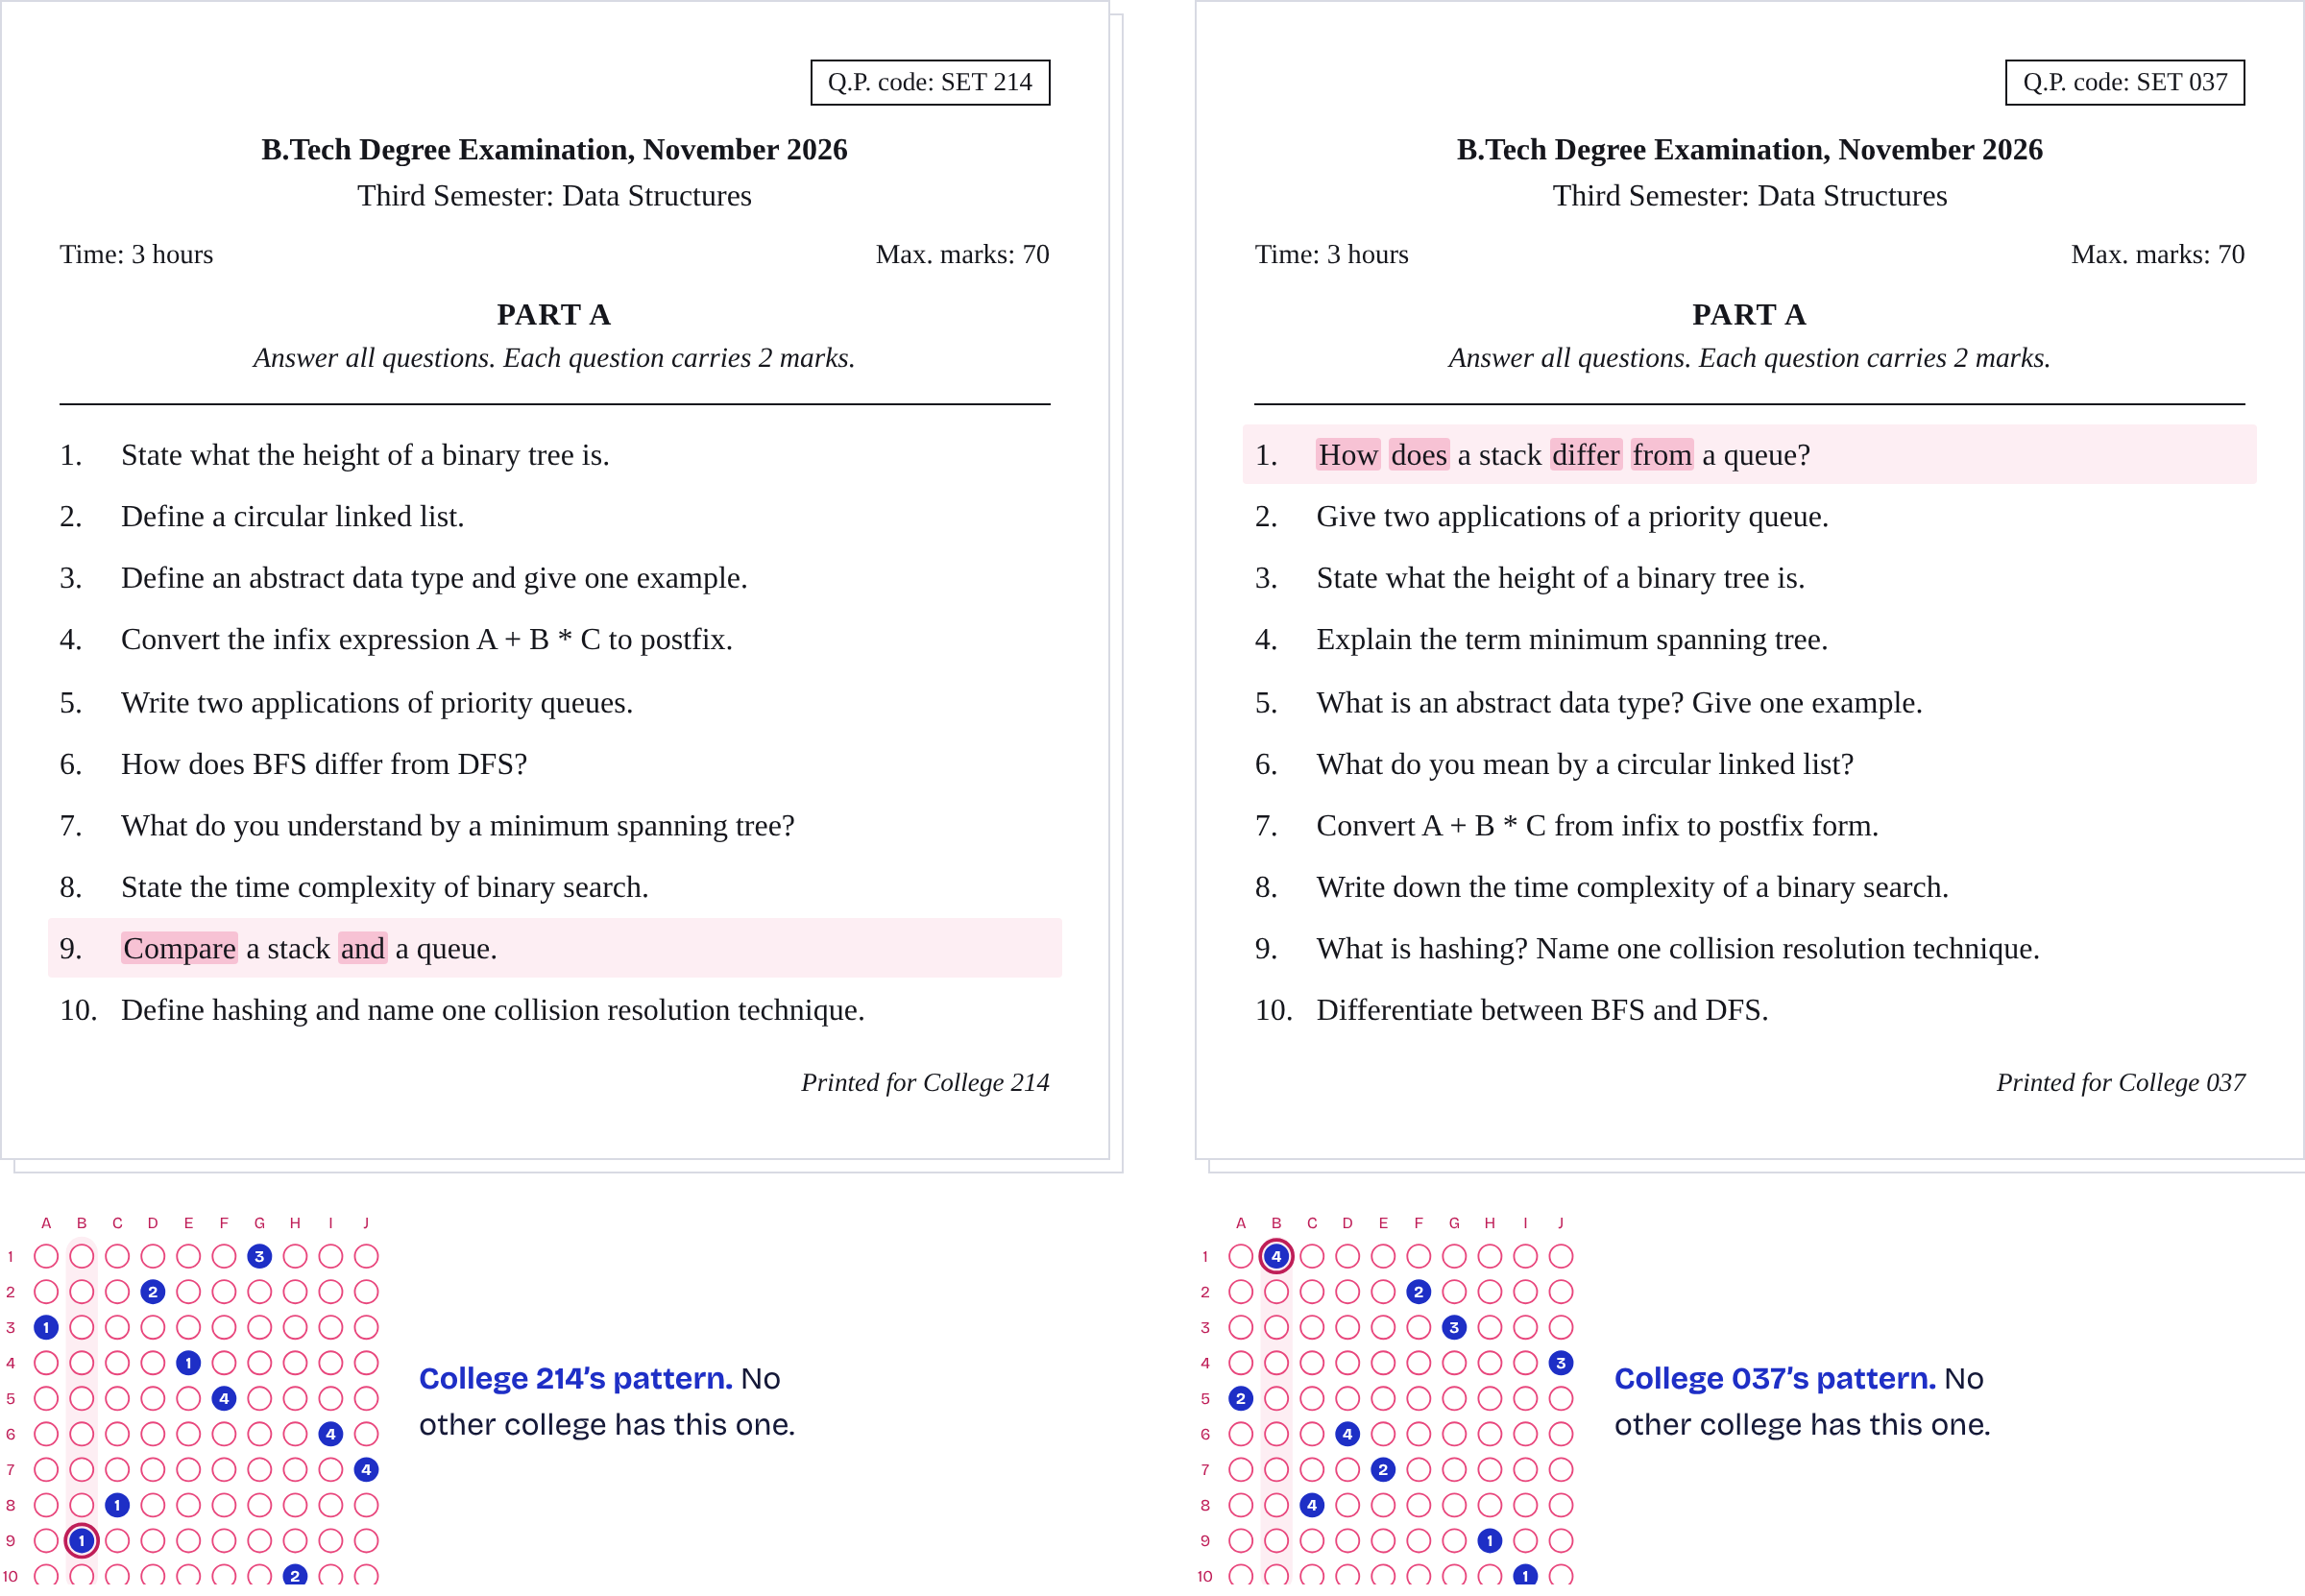
\includegraphics[width=\linewidth]{figs/papers.png}
\caption{Part A of the same Data Structures paper as printed for two colleges. The same ten questions, marks and difficulty; a different order and a different approved wording for some questions (highlighted for question B). The grids read like an OMR sheet: columns are the ten questions, rows are printed positions, and the digit in a filled bubble is the wording that college received. Screenshot of the live demo.}
\label{fig:papers}
\end{figure}

Every college receives the same questions, marks, sections and difficulty. Within limits the setter approves, three layers vary (Fig.~\ref{fig:papers}, Table~\ref{tab:layers}).

\begin{table}[t]
\centering\tablefont
\caption{What survives each attack. Layer~3 can only be erased by changing the numbers or the answers, which makes the leak wrong.}
\label{tab:layers}
\begin{tabularx}{\linewidth}{@{}Y>{\raggedright\arraybackslash}p{0.21\linewidth}>{\raggedright\arraybackslash}p{0.19\linewidth}>{\raggedright\arraybackslash}p{0.21\linewidth}@{}}
\toprule
What the leaker does & Layer 1: order & Layer 2: wording & Layer 3: numbers, answers \\
\midrule
Retypes with mistakes & survives & survives & survives \\
Sends a photo or a crop & survives & survives & survives \\
Drops or changes question numbers & relative order survives & survives & survives \\
Shuffles the lines & \textcolor{form}{erased} & survives & survives \\
Rewords every question (any tool) & survives & \textcolor{form}{erased} & survives \\
Rewords and shuffles & \textcolor{form}{erased} & \textcolor{form}{erased} & survives \\
\bottomrule
\end{tabularx}
\end{table}

\subsection{Layer 1: order}
Equal-mark short questions are permuted per college. In our Part A of $Q=10$ two-mark questions, college codewords form a permutation code in which any two colleges agree on at most 4 of the 10 positions; we build it greedily from random permutations with that rejection rule. Either/or labels and the order of sub-parts add binary symbols. Each MCQ shows its four options in one of $4!=24$ orders; we use 23 of them as symbols of GF(23) and give college $c$ the polynomial $f_c(x)=m_0+m_1x$, so question $i$ shows option order $f_c(i)$. This is a Reed--Solomon code~\citep{reed1960} with $23^2=529$ codewords of length up to 23 (we use 20), and any two colleges share at most one question's option order. Order marks are constrained (\S\ref{sec:fair}): related questions stay together and the easy-to-hard progression is kept.

\subsection{Layer 2: wording}
Each short question has $V$ faculty-approved wordings that differ in form but not meaning (\enquote{Compare a stack and a queue} / \enquote{How does a stack differ from a queue?}). We used $V=4$. Wordings must stay far enough apart that a typo cannot turn one into another; the decoder counts a wording only when a line is clearly closer to one wording than to the others (\S\ref{sec:decoder}).

\subsection{Layer 3: load-bearing marks}
\label{sec:tier3}
Layers 1 and 2 can be laundered by a leaker who rewords and shuffles every question. Layer 3 sits in content the leak cannot do without.

\paragraph{Answer keys} The letter under which each right option sits varies by college. College answer keys are codewords of a quaternary linear $[20,5,d]$ code, which we found by local search over systematic generator matrices: any two of its 1{,}023 nonzero codewords differ in at least $d=12$ of 20 positions. Because a bijection of the four letters applied at one position preserves every pairwise distance, we search per-position letter labellings for which as many keys as possible are balanced, and give the 500 colleges keys in which every letter appears 3 to 7 times out of 20 and 8 to 12 right answers sit in the middle positions B and C, the positions test-takers favour~\citep{attali2003}. The zero codeword becomes the setter's master key, which no college receives; every college key differs from it in at least 12 answers, so a leaked key that matches the master points upstream. A random codebook of the same size has closest pairs only 6 answers apart. Because an option order fixes the letter of the right answer, a paper's MCQs use either the Reed--Solomon option-order code (best when options leak with the questions) or the answer-key code (best when keys leak); we evaluate them separately. A product code, the key letter times the six orders of the three distractors, would carry both and is future work, as is deriving the key and numeric codes from the split key in our custody module.

\paragraph{Numeric values} For a numerical question the setter approves $A$ sets of values chosen to be of equal difficulty (for example two quantities with four approved values each, $A=16$), and answer keys are computed for each set. College $c$ receives one set per question from a code with a minimum-distance filter: with 8 numerical questions, any two colleges share at most 2 sets when $A=16$ and at most 1 when $A=64$. A reworded leak must keep its numbers, or its answer changes; numeric answers leaked on their own carry the same symbol.

\paragraph{A semantic marking assumption} Fingerprinting theory assumes colluders cannot alter marks where their copies agree~\citep{boneh1998}. Layer~3 replaces that with a property of the content: a leak that changes the values or the letters of the right answers gives students wrong answers, which defeats the purpose of most leaks. Layer~3 does not stop a leaker from adding noise, which the decoder tolerates, and it does not survive a leak rebuilt from memory without numbers; it makes laundering expensive.

\paragraph{How much evidence a leak carries} The decoder names a college only with evidence of at least $\ln(TN)=\ln(10^4\cdot 500)\approx 15.4$ nats (22.3 bits) against an outside copy. Table~\ref{tab:capacity} divides that by the evidence one item carries under the noise model and compares the result with the smallest leak named in simulation. The agreement suggests the decoder uses most of the evidence a leak contains.

\begin{table}[t]
\centering\tablefont
\caption{Evidence per leaked item against an outside copy (nats, when the item matches), the smallest leak that could clear 15.4 nats, and the share of simulated leaks of that size that were named.}
\label{tab:capacity}
\begin{tabularx}{\linewidth}{@{}Y r r r@{}}
\toprule
Leaked item & Evidence per item & Items needed (bound) & Named at that size \\
\midrule
Numbered Part A line (position + wording) & $\ln(0.98{\cdot}10)+\ln(0.95{\cdot}4)=3.62$ & 5 & 99.9\% (demo decoder) \\
MCQ with its options (option order) & $\ln(0.98{\cdot}24)=3.16$ & 5 & 90\% \\
Answer letter, decoder allowing 1 error in 5 & $\ln(0.8{\cdot}4)=1.16$ & 14 & 100\% (no errors) \\
Numeric value set, $A=16$ & $\ln(0.95{\cdot}16)=2.72$ & 6 & 83\% \\
Numeric value set, $A=64$ & $\ln(0.95{\cdot}64)=4.11$ & 4 & 89\% \\
\bottomrule
\end{tabularx}
\end{table}

\section{The decoder}
\label{sec:decoder}

\paragraph{Reading} Photos go through OCR (Tesseract~\citep{smith2007} in the prototype). Each line is parsed for a leading number (\enquote{Q1.}, \enquote{1)}, \enquote{1 -}). A line is matched to a master question in two steps: character-bigram Dice similarity picks the two most likely questions, then the longest-common-subsequence ratio against each of their approved wordings decides, with a minimum of 0.6. A wording counts as evidence only if the best ratio is at least 0.8 and beats the nearest other wording of the same question by $\min(0.05,\;0.4\,(1-s))$, where $s$ is the similarity between those two approved wordings; otherwise the line counts as its question but not as a wording. Answer keys are parsed as number--letter pairs.

\paragraph{Likelihoods} For college $c$ and a numbered line of question $q$ printed at position $p$ with wording $v$,
\begin{equation}
P_c(p,v\mid q)=\Big[(1-\varepsilon)\,\mathbb{1}\{p=\pi_c(q)\}+\tfrac{\varepsilon}{Q-1}\,\mathbb{1}\{p\ne\pi_c(q)\}\Big]\Big[(1-\varepsilon_V)\,\mathbb{1}\{v=w_c(q)\}+\tfrac{\varepsilon_V}{V-1}\,\mathbb{1}\{v\ne w_c(q)\}\Big],
\end{equation}
with $\varepsilon=0.02$ and $\varepsilon_V=0.05$. For unnumbered lines the order of each pair of lines counts: $1-\varepsilon_s$ if college $c$ prints them in that order, $\varepsilon_s=0.03$ otherwise. Answer letters use $1-\delta$ for a match and $\delta/3$ otherwise with $\delta=0.2$; numeric sets use $1-\varepsilon_n$ and $\varepsilon_n/(A-1)$ with $\varepsilon_n=0.05$. The \emph{outside-copy} model $P_0$ draws positions uniformly ($1/Q$), wordings uniformly ($1/V$), line orders uniformly ($1/k!$), letters uniformly ($1/4$) and value sets uniformly ($1/A$). The log-likelihood of a leak, $\ell_c$, is the sum over its items. If the numbers in a leak simply run $1,2,\dots,m$ with $m<Q$, they may be the leaker's own count, so both $P_c$ and $P_0$ become mixtures: with probability $1-\rho$ the numbers are printed positions, with probability $\rho=0.1$ only the order of the lines counts.

\paragraph{Decision} Let $\Lambda_c=e^{\ell_c-\ell_0}$ be college $c$'s likelihood ratio against an outside copy and $\tau=\ln T$ with $T=10^4$.
\begin{description}[leftmargin=1.2em,font=\normalfont\sffamily\bfseries\small]
\item[Stage 1, one source.] Name $\hat c=\arg\max_c\ell_c$ if $\ell_{\hat c}-\ell_{c'}\ge\tau$ for every other college $c'$, $\ell_{\hat c}-\ell_0\ge\tau+\ln N$, and no pair of colleges explains the leak $e^{\tau}$ times better than $\hat c$ alone.
\item[Stage 2, two sources.] Score every pair $\{a,b\}$ (including $a=b$) with a mixture in which each item comes from $a$ or $b$ with probability $\tfrac12$. Name a member $m$ of the best pair if that pair beats the outside-copy model by $\tau+\ln\tfrac{N(N+1)}{2}$, beats every pair without $m$ by $\tau$, and $m$'s partner's share could not come from an outside copy (a margin of $\tau+\ln N$).
\item[Otherwise] abstain and rank colleges by posterior probability under a uniform prior.
\end{description}
Stage 1 costs $O(Nk)$ and stage 2 $O(N^2k)$ for a leak of $k$ items; for $N=500$ that is 125{,}250 pairs, under a second in browser JavaScript. Answer keys use stage 1 with the master key as an extra candidate, $N+1$ in all; numeric value sets use stage 1.

\section{Guarantees}
\label{sec:guarantee}

\begin{proposition}[Outside copies]\label{prop:outside}
If a leak $X$ is drawn from the outside-copy model $P_0$, then for any $T>0$
\[
\pr_0\Big(\exists c\in\{1,\dots,N\}:\ \Lambda_c(X)\ge NT\Big)\le\frac1T .
\]
\end{proposition}
\begin{proof}
For each $c$, $\E_0[\Lambda_c(X)]=\sum_x P_0(x)\,P_c(x)/P_0(x)\le\sum_x P_c(x)\le1$ (the order model is sub-normalised). By Markov's inequality $\pr_0(\Lambda_c\ge NT)\le 1/(NT)$, and a union bound over the $N$ colleges gives $1/T$.
\end{proof}

\begin{proposition}[Anytime validity]\label{prop:anytime}
Let the items of a leak be read one at a time, $X_1,X_2,\dots$, and let $P_c(\cdot\mid X_{1:t-1})$ and $P_0(\cdot\mid X_{1:t-1})$ be the decoder's sequential models. If the leak follows $P_0$, then
\[
\pr_0\Big(\exists t\ \exists c:\ \Lambda_c(X_{1:t})\ge NT\Big)\le\frac1T .
\]
\end{proposition}
\begin{proof}
Each $\Lambda_c(X_{1:t})$ is a nonnegative $P_0$-martingale with initial value 1~\citep{ramdas2023}, so their average
\[ M_t=\frac1N\sum_{c=1}^{N}\Lambda_c(X_{1:t}) \]
is too. Ville's inequality~\citep{ville1939} gives $\pr_0(\sup_t M_t\ge T)\le 1/T$, and if some $\Lambda_c(X_{1:t})\ge NT$ then $M_t\ge T$.
\end{proof}

\noindent Investigators may therefore re-run the decoder each time another line or screenshot turns up without raising the chance of naming a college for an outside copy above $1/T$. Mixtures (over numbering readings, or over error rates) are proper likelihoods, so both propositions apply to them. Stage 2's pair test uses $N(N+1)/2$ pairs in place of $N$ and is bounded by $1/T$ in the same way, so for the full two-stage decoder a union bound gives $2/T$; answer keys use stage 1 only.

\begin{proposition}[Separation by code distance]\label{prop:distance}
Suppose a leak reproduces college $a$'s marks without error on $k$ items. (i) MCQs with options, Reed--Solomon code: every other college matches at most one item, so $\ell_a-\ell_b\ge(k-1)\ln\frac{23(1-\varepsilon)}{\varepsilon}=7.03\,(k-1)$ nats, which exceeds $\tau$ for $k\ge3$. (ii) Answer keys from the $[20,5,12]$ code with $n=20$ answers: any other key disagrees with $a$'s on at least $k-8$ of the $k$ leaked answers, so $\ell_a-\ell_b\ge(k-8)\ln\frac{3(1-\delta)}{\delta}=2.48\,(k-8)$ nats, which exceeds $\tau$ for $k\ge12$; each wrong answer in the leak costs at most $2\ln12=4.97$ nats of that margin.
\end{proposition}
\begin{proof}
(i) Two Reed--Solomon codewords $m_0+m_1x$ agree on at most one $x$. (ii) Two keys differ in at least 12 of 20 positions, of which at most $20-k$ lie outside the leak. Each disagreement contributes $\ln\frac{1-\delta}{\delta/3}$ to $\ell_a-\ell_b$ and each agreement 0; an error turns one term from $+\ln12$ to at least $-\ln12$.
\end{proof}

\paragraph{What is and is not guaranteed} Propositions~\ref{prop:outside}--\ref{prop:anytime} bound wrong names for outside copies under the outside-copy model; Section~\ref{sec:evalg} checks them empirically for numbered Part A lines and answer keys only, and the attack test of Section~\ref{sec:eval} covers the full decoder on outside copies (1 of 32{,}000 named). They do not bound misattribution between colleges. For a leak that did come from some college, the runner-up test makes the named college at least $T$ times likelier than every other; under a uniform prior over colleges its posterior probability is then at least $1/(1+(N-1)/T)\ge95.2\%$ for $N=500$, and in practice far higher because most colleges are excluded by many orders of magnitude. A frequentist bound per wrong college, $\pr_a(\Lambda_b/\Lambda_a\ge T)\le 1/T$, sums only to $(N-1)/T\approx5\%$, which is why the codes' distances matter (Proposition~\ref{prop:distance}) and why we report misattribution empirically. Requiring $TN$ against the runner-up as well would make that bound $1/T$ at the cost of about one or two more leaked lines. The guarantee also assumes the outside-copy model is right; Section~\ref{sec:evalg} shows one place where real copies differ from it.

\section{Custody and integrity}
\label{sec:custody}

A tracing system is only as trustworthy as the people who hold its keys. Our design removes single points of misuse (implemented in \texttt{custody.py}, 12 of 12 self-checks pass).
\begin{enumerate}[label=(\alph*)]
\item \textbf{No single key-holder.} The master key is split into three shares with Shamir's scheme over the prime field $2^{521}-1$~\citep{shamir1979}; any two officials (for example the Controller of Examinations, the Registrar and an outside observer) can rebuild it, and one alone learns nothing.
\item \textbf{No stored table.} Every college's codeword is derived from the key with HMAC-SHA256~\citep{rfc2104} as the random generator while keeping each code's structure (at most 4 shared positions; at most one shared option order). The college-to-pattern table exists only while two share-holders are present; deriving all 500 codewords takes about 0.6\,s.
\item \textbf{A fingerprint that leaves the building.} All per-college PDFs are hashed into one Merkle root~\citep{merkle1987} with RFC~6962 leaf and node prefixes~\citep{rfc6962}, signed by two officials with Ed25519~\citep{bernstein2012} and sent to every principal before the exam. Each college can later prove which file it received, and nobody can swap a paper afterwards without the published root exposing it. No single official can therefore frame a college or swap a paper undetected; two colluding key-holders could still leak a chosen college's paper, which is why the log and the inquiry, not the decoder alone, decide.
\item \textbf{A hash-chained log} of every generation and decoding, for audit.
\end{enumerate}
An attribution is a lead, not a verdict. It should be reported with its likelihood ratios and the features that matched, used to decide which phones and logs to examine, and confirmed by other evidence; used in court it would be expert evidence about an electronic record under the Bharatiya Sakshya Adhiniyam, 2023.

\section{Evaluation}
\label{sec:eval}

\subsection{Setup}
All experiments use $N=500$ simulated colleges, $T=10^4$ ($\tau=9.21$ nats) and fixed seeds. The paper is a Data Structures paper: Part A has ten two-mark questions with four approved wordings each; Part B has either/or pairs with two sub-parts; 20 MCQs carry option orders. Typing damage deletes, replaces or doubles characters at 4\% unless stated, and half the lines are lower-cased with punctuation removed. Code and outputs are in the public repository (Appendix~\ref{app:repro}).

\subsection{Whole-paper simulation}
Figure~\ref{fig:channels} shows the share of leaks named, and the share with the real source in a top-5 shortlist, by number of leaked items (3{,}000 leaks per point). Numbered leaks with wording variants are named from 5 questions in 36\% of leaks, 6 in 74\%, 7 in 92\% and 8 in 97\%; from 4 questions the source is in the top 5 in 99.9\%. MCQs with options are named from 5 questions in 90\%. Unnumbered leaks need more: 51\% at 8 questions and 84\% at 10 with wording variants. These leaks draw items from the whole paper, Part A and Part B; Part B items carry less evidence each, so they need more items than the Part-A-only leaks of Table~\ref{tab:attack}. No honest single-source leak was pinned on an innocent college in 135{,}000 leaks, and none of 135{,}000 outside copies was named.

\begin{figure}[t]
\centering
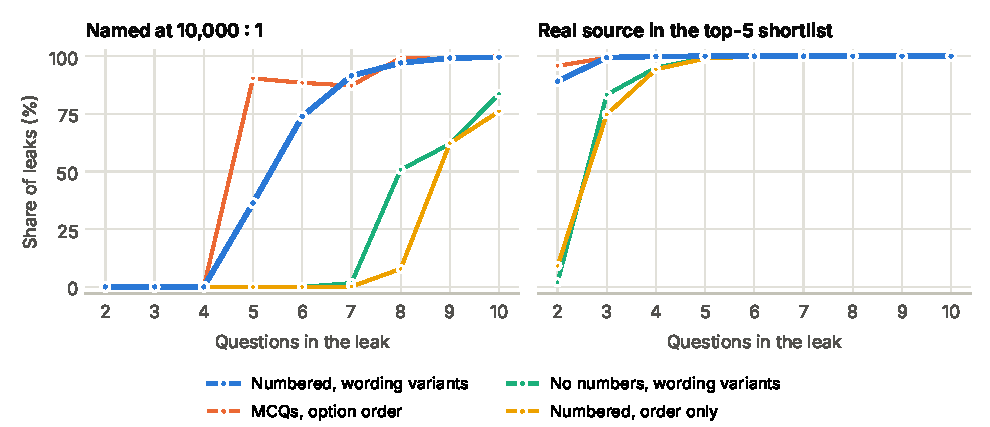
\includegraphics[width=\linewidth]{figs/channels.pdf}
\caption{Whole-paper simulation, 500 colleges, 3{,}000 leaks per point. Left: leaks named at 10{,}000 to 1. Right: leaks whose real source is in the top-5 shortlist (ties counted against us).}
\label{fig:channels}
\end{figure}

\subsection{End to end, through OCR}
We rendered college pages, damaged them like phone photos forwarded on WhatsApp (crops showing 3--6 questions, rotation, perspective, blur, noise, downscaling and JPEG compression) and decoded them through Tesseract. Of 80 photos, 99.4\% of visible questions were recovered. All 30 photos showing 5 or 6 questions were named, all correctly; photos showing 4 questions were never named but had the source in the top 5 every time (26 of 26), and 3-question photos in 96\% (23 of 24). No photo was pinned on an innocent college.

\subsection{Adversarial sweep}
We attacked the decoder that runs in the public demo with 148{,}000 simulated leaks in 74 settings (Table~\ref{tab:attack}). Tricks can stop it naming anyone; they did not make it name an innocent college, with one exception: an outside copy of six numbered lines whose positions all matched one college and whose wordings matched five of six. Before we hardened the decoder (weighing both readings of numbers that run 1, 2, 3; gating wordings; raising the bar from 1{,}000 to 10{,}000), the same leaks named eight innocent colleges. A separate count over one million random outside copies per length bounds the chance that some college clears the outside-copy bar at about 1 in 20{,}000 (6 lines), the peak over lengths. Under heavier typing damage, 5 numbered lines are still named in 99.2\% of leaks at 15\% character damage and 95.8\% at 20\%; 7 unnumbered lines in 99.7\% and 93.2\%. No innocent college was named in any of the 70{,}000 leaks of the damage tests (0--40\% of characters damaged).

\begin{table}[t]
\centering\tablefont
\caption{Adversarial sweep of the demo decoder, 2{,}000 leaks per setting, typing damage at 4\% of characters except in the damage row. \enquote{Named from} is the smallest leak named in at least 95\% of cases.}
\label{tab:attack}
\begin{tabularx}{\linewidth}{@{}Y>{\raggedleft\arraybackslash}p{0.25\linewidth}>{\raggedleft\arraybackslash}p{0.13\linewidth}>{\raggedleft\arraybackslash}p{0.15\linewidth}@{}}
\toprule
What the leaker did & Named from & In top 5, 6 lines & Innocent named \\
\midrule
Kept the printed numbers & 5 lines & 100\% & 0 of 12{,}000 \\
Left the numbers out & 7 lines & 100\% & 0 of 12{,}000 \\
Renumbered the lines 1, 2, 3 & 7 lines & 100\% & 0 of 12{,}000 \\
Copied the first questions (real numbers 1, 2, 3) & 6 lines & 100\% & 0 of 8{,}000 \\
Reworded every question, kept numbers & holds back (61\% at 10) & 99.8\% & 0 of 12{,}000 \\
Reworded every question, no numbers & holds back & 56.3\% & 0 of 12{,}000 \\
Shuffled the lines, no numbers & holds back & 31.4\% & 0 of 12{,}000 \\
Mixed two colleges' copies, numbered & 10 lines & $>$99.9\% & 0 of 6{,}000 \\
Mixed two colleges' copies, no numbers & holds back (3\% at 10) & 88.8\% (10 lines) & 0 of 2{,}000 \\
Sent a copy from outside the system & -- & -- & 1 of 32{,}000 \\
Typing damage 0--40\%, 6 lines (14 settings) & see text & $\ge$99.9\% & 0 of 28{,}000 \\
\midrule
All 74 settings & & & 1 of 148{,}000 \\
\bottomrule
\end{tabularx}
\end{table}

\subsection{Mixed copies}
When each leaked item comes at random from one of two colleges' copies, the two-stage decoder of the Python reference names only real sources in 59\% of 10-question numbered leaks and 87\% of 12-question ones, and in 83\% of 10-MCQ leaks; with fewer items it mostly abstains, with a real source in the top 5 for 88--100\%. No innocent college was named in 45{,}000 mixed leaks, 15{,}000 single-source leaks or 15{,}000 outside copies with both stages on. At the old 1{,}000-to-1 bar two mixes framed a third college whose random Part~A wording variants happened to match; structured codes are the fix. For MCQs, the Reed--Solomon code rules framing out for two colluders once five or more MCQs leak without misreads, the traceability condition $d>n(1-1/c^2)$~\citep{staddon2001}, and it named no innocent college in 26{,}000 leaks (nor did a random codebook in another 26{,}000). Part~A's ten positions are too few to meet that condition, so a structured code for wordings is future work.

\subsection{Layer 3: answer keys and numeric values}
Figure~\ref{fig:tier3} and Table~\ref{tab:tier3} summarise 3{,}000 leaks per point. A key with no wrong answers is named from 14 answers every time; with one wrong answer in ten, 20 answers are named in 87\% of keys; with one in five, 41\%. Below those sizes the source stays near the top: from 8 answers with one error in ten it is in the top 5 for 95.4\% of keys. Leaks of the master key (16 answers, one error in ten) were traced upstream in 52\% and never pinned on a college. The random codebook names about as often but its closest keys are only 6 answers apart, against 12 for the code. For numeric values, after rewording and shuffling so that only the numbers survive (3\% of numbers misread), 16 approved sets per question name the source from 6 questions in 83\% of leaks and from 8 in 98\%; 64 sets name it from 4 questions in 89\%. With 4 sets nothing is named, but the source is in the top 5 for at least 98\% of 6-question leaks. Naming is not monotone at the margin (83\% at 6, 80\% at 7) because one misread value costs about two questions' worth of evidence ($2.72+2.93=5.65$ nats), so these rates are close to $0.97^6$ and $0.97^7$, the chance that no value is misread. No innocent college was named in 171{,}000 layer-3 leaks.

\begin{figure}[t]
\centering
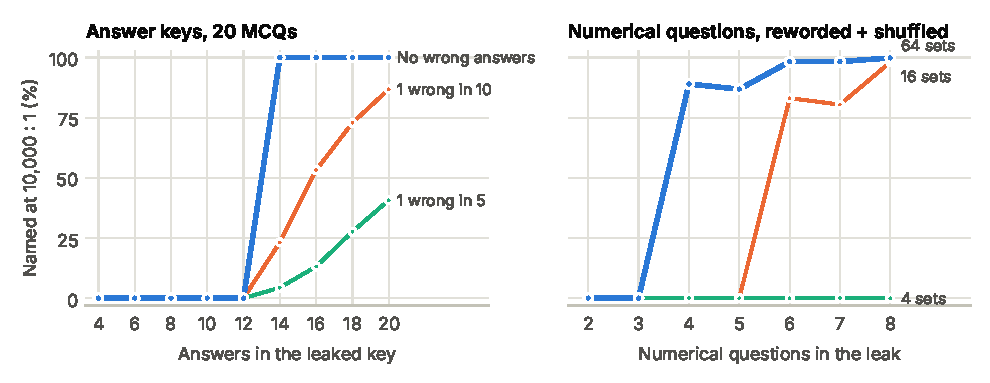
\includegraphics[width=\linewidth]{figs/tier3.pdf}
\caption{Layer 3, 500 colleges, 3{,}000 leaks per point. Left: answer keys from the $[20,5,12]$ code, by number of leaked answers and share of wrong answers. Right: numerical questions reworded and shuffled so that only their values survive, by number of approved value sets per question.}
\label{fig:tier3}
\end{figure}

\begin{table}[t]
\centering\tablefont
\caption{Layer 3 summary (3{,}000 leaks per cell). Top 5 counts ties against us.}
\label{tab:tier3}
\begin{tabularx}{\linewidth}{@{}Y r r r@{}}
\toprule
Leak & Named & Real source in top 5 & Innocent named \\
\midrule
Answer key, 14 answers, no errors & 100\% & 100\% & 0 \\
Answer key, 20 answers, 1 error in 10 & 86.8\% & 100\% & 0 \\
Answer key, 8 answers, 1 error in 10 & 0\% & 95.4\% & 0 \\
Answer key, 20 answers, 1 error in 5 & 40.7\% & 99.9\% & 0 \\
Setter's master key, 16 answers, 1 error in 10 & traced upstream 52.1\% & -- & 0 \\
Numeric, 16 sets, 6 questions, reworded and shuffled & 83.1\% & 100\% & 0 \\
Numeric, 16 sets, 8 questions & 98.1\% & 100\% & 0 \\
Numeric, 64 sets, 4 questions & 89.0\% & $>$99.9\% & 0 \\
\midrule
All 171{,}000 layer-3 leaks (code keys and numeric) & & & 0 \\
\bottomrule
\end{tabularx}
\end{table}

\subsection{The guarantee, checked}
\label{sec:evalg}
We read 800{,}000 outside copies one item at a time: 200{,}000 numbered Part A copies drawn from the decoder's own outside-copy model, 200{,}000 realistic Part A copies and 400{,}000 answer keys, and counted how often \emph{any} college's ratio ever reached $TN$ (Fig.~\ref{fig:guarantee}). This checks the single-college test for these two channels; the attack test above covers the full decoder. For outside copies drawn from the decoder's own model the rate stays under $1/T$ at every bar ($5\times10^{-6}$ at $T=10^4$). For realistic copies, whose printed positions form a permutation rather than independent draws, the rate is $5.5\times10^{-5}$ at $T=10^4$ (11 of 200{,}000), inside the bound, but at $T=100$ it is 1.13\%, slightly above the 1\% the model promises, because positions drawn without replacement match a college's pattern a little more often than independent ones. Answer keys stay inside the bound everywhere ($3.5\times10^{-5}$ at $T=10^4$, 14 of 400{,}000). At $T=10^4$ the realistic Part A rate is within a factor of two of the bound, so the model matters. Crossing the outside-copy bar is necessary but not sufficient to be named, since the runner-up test must also pass. Figure~\ref{fig:trajectory} shows two sequential reads.

\begin{figure}[t]
\centering
\begin{minipage}[t]{0.52\linewidth}\vspace{0pt}
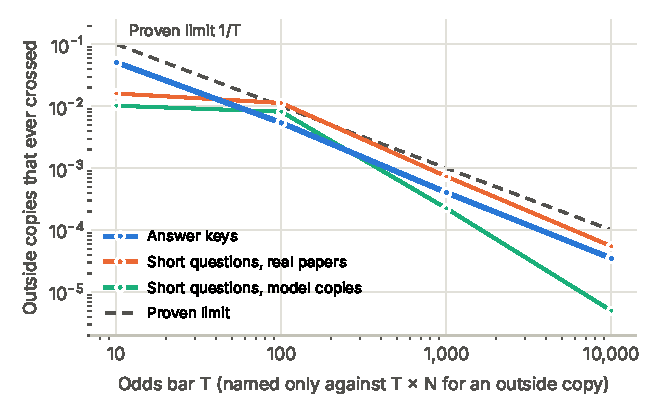
\includegraphics[width=\linewidth]{figs/guarantee.pdf}
\end{minipage}\hfill
\begin{minipage}[t]{0.45\linewidth}\vspace{6pt}
\caption{Share of outside copies for which some college's likelihood ratio ever reached $T\times N$ while the copy was read item by item, against the proven limit $1/T$ (Proposition~\ref{prop:anytime}). Model copies follow the decoder's outside-copy model; real papers draw positions as a permutation, which exceeds the model's bound slightly at $T=100$. At the bar we use, $T=10^4$, all three stay inside it.}
\label{fig:guarantee}
\end{minipage}
\end{figure}

\begin{figure}[t]
\centering
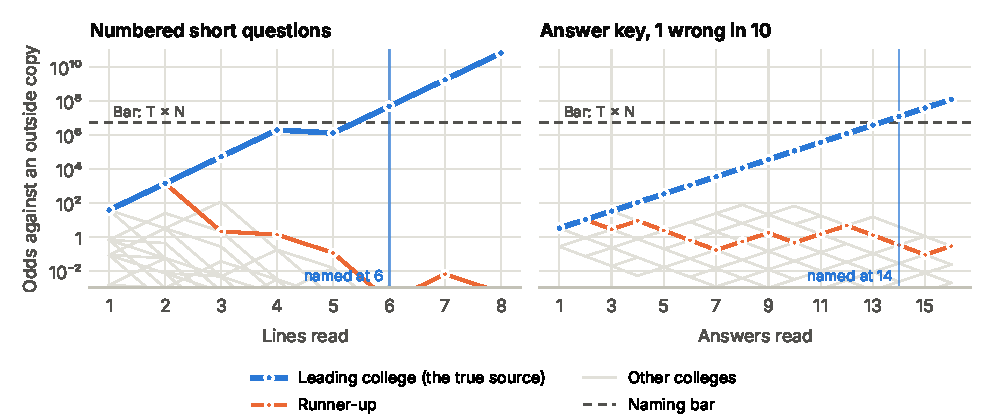
\includegraphics[width=\linewidth]{figs/trajectory.pdf}
\caption{Evidence growing as a leak is read. Left: eight numbered short questions from one college; the source crosses the bar and leads every other college by $10^4$ at line 6. Right: a 16-answer key with one wrong answer in ten; named at answer 14. Grey lines are the next 38 colleges.}
\label{fig:trajectory}
\end{figure}

\subsection{Runtime}
Decoding a leak against 500 colleges, including the $N^2/2$ pair stage, takes well under a second in browser JavaScript on a laptop; the live demo runs 200 leaks in a few seconds. Deriving 500 codewords from the key takes about 0.6\,s in Python.

\section{Fairness and deployment}
\label{sec:fair}
\label{sec:deploy}

\paragraph{Fairness constraints} Following the evidence in Section~\ref{sec:related}: we permute only within equal-mark blocks, either/or pairs, sub-parts and MCQ options, where we expect order to matter least; keep related questions adjacent and the easy-to-hard order fixed; have a faculty member approve every wording and value set; balance every answer key (3--7 of each letter, 8--12 middle answers); and generate answer keys per version so valuers mark against the right key, with the version ID printed for them. Numeric value sets must be equivalent in steps and arithmetic, and because facility can still differ~\citep{westacott2023}, a pilot should calibrate them before high-stakes use. After every exam the university publishes mean marks per version; a version that scores differently is visible at once.

\paragraph{Fit with delivery} Only one step changes: the moment a university makes each college's PDF. Colleges download and print as today. For computer-based tests, which NEET moves to from 2027~\citep{quint2026cbt}, a different arrangement per centre or per candidate costs nothing, and a phone photo of a screen is traced the same way. Last-minute generation from a verified question bank, as recently proposed~\citep{bs2026nilekani,iiith2026}, is compatible: per-centre versions are made at the same moment.

\paragraph{Side effect} Because any two colleges' answer keys differ in at least 12 of 20 answers, a key leaked from one college is mostly wrong at every other college. This contains the damage of the answer relays seen in recruitment exams~\citep{tnm2023tspsc}, independently of tracing.

\paragraph{Cost and pilot} The software is open source and runs on a laptop; the main recurring cost is setter time to write two or three wordings or value sets per question. Our plan: a campus leak lab and student survey (November 2026), a per-college PDF generator with answer keys (December), a pilot in one college's internal exams with one version per hall (next semester), then one university exam series.

\section{Limitations}
\label{sec:limits}
\begin{itemize}
\item \textbf{Synthetic evaluation.} Pages, damage and leaker behaviour are simulated. How often real leakers renumber, reword or shuffle ($\rho$ and the attack mix) is unknown until the leak lab.
\item \textbf{Upstream leaks.} Leaks at the setters or the press, as in NEET-UG 2026~\citep{tribune2026cbi}, cannot be pinned on a college. For answer keys Leak Trace recognises them as matching the master key; for question text it abstains.
\item \textbf{Laundered leaks.} A leaker who rewords and shuffles every short question erases layers 1 and 2. Without numerical questions or an answer key the decoder abstains; it does not guess. A paper rebuilt from memory, like a \enquote{guess paper}, keeps little structure.
\item \textbf{Answer keys as text.} A key written as answer texts instead of letters loses the letter channel, though the option texts then carry layer 1.
\item \textbf{Collusion.} Two-copy mixes are handled; larger coalitions would need far longer codes than one paper offers~\citep{tardos2008}.
\item \textbf{Misattribution bound.} The $1/T$ bound covers outside copies; between colleges we give a posterior bound and empirical counts (\S\ref{sec:guarantee}).
\item \textbf{Languages and OCR.} English only. Tesseract ships Telugu, Kannada, Tamil and Malayalam models, untested here; vision-language OCR may normalise wording and blur layer 2.
\item \textbf{Law and practice.} No Indian court has considered a statistical attribution of a leaked paper; the output is designed as an investigative lead.
\end{itemize}

\section{Conclusion}
Paper leaks in India are detected quickly and attributed slowly. Leak Trace moves attribution to the moment a leak is seen, by printing each college's identity into the content of a fair paper and reading it back with a decoder that states its own error rate and refuses to guess. The third layer of marks, numbers and answers, is the strongest: a leaker cannot remove it without making the leaked answers wrong. The next step is real data: a leak lab with our classmates, then a pilot in one college's internal exams.

\section*{Acknowledgements}
We thank our faculty and the coordinators of the Seva First Innovation Challenge at our institute.

\appendix
\section{Parameters}
\begin{table}[H]
\centering\tablefont
\begin{tabularx}{\linewidth}{@{}l Y@{}}
\toprule
Parameter & Value \\
\midrule
Colleges $N$, naming bar $T$ & 500; $10^4$ ($\tau=9.21$ nats; outside-copy margin $\tau+\ln N=15.4$ nats) \\
Part A & $Q=10$ positions, permutation code with at most 4 shared positions; $V=4$ wordings \\
Noise & position $\varepsilon=0.02$; wording $\varepsilon_V=0.05$; pair order $\varepsilon_s=0.03$; own-numbering prior $\rho=0.1$ \\
Matching & bigram Dice for the top 2 questions, LCS ratio $\ge0.6$; wording counts if $r\ge0.8$ and margin $\ge\min(0.05,0.4(1-s))$ \\
MCQs & 20 questions, Reed--Solomon over GF(23), $f_c(x)=m_0+m_1x$ \\
Answer keys & quaternary $[20,5,12]$ linear code, per-position letter labelling, 3--7 of each letter, 8--12 in B/C; $\delta=0.2$ \\
Numeric values & 8 questions; $A\in\{4,16,64\}$ with at most 5, 2, 1 shared sets; $\varepsilon_n=0.05$ \\
Custody & Shamir 2-of-3 over $2^{521}-1$; HMAC-SHA256; RFC 6962 Merkle tree; Ed25519 \\
\bottomrule
\end{tabularx}
\end{table}

\section{Reproducibility}
\label{app:repro}
Live demo (runs the decoder in the browser):\\
\url{https://raw.githack.com/SakethSumanBathini/SakethSumanBathini/leak-trace-site/index.html}\\
Code, seeds and result files: \url{https://github.com/SakethSumanBathini/SakethSumanBathini/tree/leak-trace-site}\\
\texttt{sim\_decode.py} (whole paper), \texttt{e2e\_ocr.py} (OCR), \texttt{sim\_coalition.py} (mixes), \texttt{sim\_rs\_mcq.py} (Reed--Solomon), \texttt{sim\_tier3.py} (answer keys, numeric values, guarantee check), \texttt{adversarial/sweep.js} (attack sweep on the demo decoder), \texttt{custody.py} (key custody, 12 self-checks). Results quoted here are in \texttt{results/} and \texttt{adversarial/runs/}.

\FloatBarrier
\small
\begin{thebibliography}{99}

\bibitem[Newslaundry(2024)]{newslaundry2024} Newslaundry. \enquote{10 years, 89 paper leak cases, 48 retests: from Centre to states, few plugs for a leaky record.} 31 July 2024. \url{https://newslaundry.com/2024/07/31/10-years-89-paper-leak-cases-48-retests-from-centre-to-states-few-plugs-for-a-leaky-record}

\bibitem[Moneylife(2026)]{moneylife2026} Moneylife. \enquote{NEET-UG 2026 cancelled over paper leak allegations; re-exam to be held, CBI probe ordered.} 12 May 2026. \url{https://moneylife.in/article/neetug-2026-cancelled-over-paper-leak-allegations-reexam-to-be-held-cbi-probe-ordered/80438.html}

\bibitem[SouthFirst(2025)]{southfirst2025kannur} South First. \enquote{College principal suspended as Kannur University exam paper leak case deepens.} 20 April 2025. \url{https://thesouthfirst.com/news/college-principal-suspended-kannur-university-exam-paper-leak-case-deepens/}

\bibitem[ETV Bharat(2025)]{etv2025bu} ETV Bharat. \enquote{Bangalore University to send B.Ed exam question papers online to prevent leaks.} February 2025. \url{https://www.etvbharat.com/en/!state/bangalore-university-to-send-bed-exam-question-papers-online-to-prevent-leaks-enn25022103978}

\bibitem[Udayavani(2018)]{udayavani2018vtu} Udayavani. \enquote{VTU orders probe into leak of papers.} 16 June 2018. \url{https://www.udayavani.com/english-news/vtu-orders-probe-into-leak-of-papers}

\bibitem[JNTUH(2019)]{jntuh2019aqar} JNTU Hyderabad. Annual Quality Assurance Report 2018--19 (NAAC), listing \enquote{Electronic Distribution of Examination Papers (EDEP)}. \url{https://jntuh.ac.in/uploads/downloads/NAAC_AQAR_201819.pdf}

\bibitem[JNTUH(2018)]{jntuh2018news} JNTU Hyderabad, Directorate of Evaluation. Newsletter 2017--18 (students \enquote{jumbled cluster wise and mapped to host colleges}). \url{https://jntuh.ac.in/uploads/newsletters/DE2018.pdf}

\bibitem[Onmanorama(2025)]{onmanorama2025b} Onmanorama. \enquote{Bekal police book Kasaragod college principal for leaking BCA questions to students.} 19 April 2025. \url{https://onmanorama.com/news/kerala/2025/04/19/bekal-police-book-kasaragod-college-principal-leaking-bca-questions-students.html}

\bibitem[Deccan Herald(2025)]{dh2025kslu} Deccan Herald. \enquote{Law college vice-principal among three arrested for exam paper leak.} 18 February 2025. \url{https://www.deccanherald.com/amp/story/india%2Fkarnataka%2Fbengaluru%2Flaw-college-vice-principal-among-three-arrested-for-exam-paper-leak-2-3410420}

\bibitem[Tribune(2023)]{tribune2023haryana} The Tribune. \enquote{To check paper leak, board question papers to now have QR code.} February 2023. \url{https://www.tribuneindia.com/news/haryana/to-check-paper-leak-board-question-papers-to-now-have-qr-code-481413/amp}

\bibitem[Deccan Herald(2024)]{dh2024wbbse} Deccan Herald. \enquote{Bengal secondary board introduces secret code in question paper.} 2024. \url{https://www.deccanherald.com/amp/story/india%2Fwest-bengal%2Fbengal-secondary-board-introduces-secret-code-in-question-paper-2875702}

\bibitem[Sakshi Post(2025)]{sakshi2025tsssc} Sakshi Post. \enquote{Telangana SSC question papers have QR codes and security numbers to prevent leakage.} 2025. \url{https://www.sakshipost.com/news/telangana/telangana-ssc-question-papers-have-qr-codes-and-security-numbers-prevent-leakage}

\bibitem[NIOS(2026)]{nios2026} National Institute of Open Schooling. Theory exam centre question-paper download presentation, 28 March 2026. \url{https://exams.nios.ac.in/static/docs/NIOS_TheoryExamCentre_QPDownload_Presentation_Tricolor_28March2026.pdf}

\bibitem[Siasat(2026)]{siasat2026pjtsau} Siasat. \enquote{Telangana agricultural university exam paper leaked; 4 staff suspended.} 9 January 2026. \url{https://www.siasat.com/telangana-agricultural-university-exam-paper-leaked-4-staff-suspended-3323281/amp/}

\bibitem[The Week(2026)]{theweek2026neet} The Week. \enquote{How the NEET paper leak was exposed by a hostel owner and a teacher in Rajasthan.} 13 May 2026. \url{https://www.theweek.in/news/india/2026/05/13/how-the-neet-paper-leak-was-exposed-by-a-hostel-owner-and-a-teacher-in-rajasthan.amp.html}

\bibitem[Tribune(2026)]{tribune2026cbi} The Tribune. \enquote{NEET paper leak: 3 NTA subject experts primary sources of leak, says CBI chargesheet.} 7 August 2026. \url{https://www.tribuneindia.com/news/india/neet-paper-leak-3-nta-subject-experts-primary-sources-of-leak-says-cbi-chargesheet/}

\bibitem[Boneh and Shaw(1998)]{boneh1998} D.~Boneh and J.~Shaw. Collusion-secure fingerprinting for digital data. \emph{IEEE Transactions on Information Theory}, 44(5):1897--1905, 1998.

\bibitem[Reed and Solomon(1960)]{reed1960} I.~S. Reed and G.~Solomon. Polynomial codes over certain finite fields. \emph{Journal of the SIAM}, 8(2):300--304, 1960. doi:10.1137/0108018.

\bibitem[Wikipedia(2026)]{wiki_canary} Wikipedia. Canary trap. Accessed October 2026. \url{https://en.wikipedia.org/wiki/Canary_trap}

\bibitem[Fingas(2019)]{engadget2019genius} J.~Fingas. Genius accuses Google of copying its lyrics data. \emph{Engadget}, 16 June 2019.

\bibitem[Krulwich(2014)]{npr2014agloe} R.~Krulwich. An imaginary town becomes real, then not. True story. NPR, 18 March 2014.

\bibitem[OUP(2005)]{oup2005} Oxford University Press blog. NOAD on Boing-Boing. October 2005.

\bibitem[Brassil et~al.(1995)]{brassil1995} J.~Brassil, S.~Low, N.~F. Maxemchuk and L.~O'Gorman. Electronic marking and identification techniques to discourage document copying. \emph{IEEE Journal on Selected Areas in Communications}, 13(8):1495--1504, 1995.

\bibitem[EchoMark(2026)]{echomark2026} EchoMark. US Patent 12,620,252 B2, granted 5 May 2026. \url{https://patents.google.com/patent/US12620252B2/en}

\bibitem[Atallah et~al.(2001)]{atallah2001} M.~J. Atallah, V.~Raskin, M.~Crogan, C.~Hempelmann, F.~Kerschbaum, D.~Mohamed and S.~Naik. Natural language watermarking: design, analysis, and a proof-of-concept implementation. In \emph{Information Hiding 2001}, LNCS 2137. doi:10.1007/3-540-45496-9\_14.

\bibitem[Topkara et~al.(2006)]{topkara2006} U.~Topkara, M.~Topkara and M.~J. Atallah. The hiding virtues of ambiguity: quantifiably resilient watermarking of natural language text through synonym substitutions. In \emph{ACM Multimedia and Security Workshop}, 2006.

\bibitem[Yang et~al.(2022)]{yang2022} X.~Yang, J.~Zhang, K.~Chen, W.~Zhang, Z.~Ma, F.~Wang and N.~Yu. Tracing text provenance via context-aware lexical substitution. In \emph{AAAI}, 2022. arXiv:2112.07873.

\bibitem[Kirchenbauer et~al.(2023)]{kirchenbauer2023} J.~Kirchenbauer, J.~Geiping, Y.~Wen, J.~Katz, I.~Miers and T.~Goldstein. A watermark for large language models. In \emph{ICML}, PMLR 202:17061--17084, 2023.

\bibitem[Kirchenbauer et~al.(2024)]{kirchenbauer2024} J.~Kirchenbauer et~al. On the reliability of watermarks for large language models. In \emph{ICLR}, 2024.

\bibitem[Dathathri et~al.(2024)]{dathathri2024} S.~Dathathri, A.~See, S.~Ghaisas et~al. Scalable watermarking for identifying large language model outputs. \emph{Nature}, 634:818--823, 2024. doi:10.1038/s41586-024-08025-4.

\bibitem[Krishna et~al.(2023)]{krishna2023} K.~Krishna, Y.~Song, M.~Karpinska, J.~Wieting and M.~Iyyer. Paraphrasing evades detectors of AI-generated text, but retrieval is an effective defense. In \emph{NeurIPS} 36:27469--27500, 2023.

\bibitem[Chor et~al.(1994)]{chor1994} B.~Chor, A.~Fiat and M.~Naor. Tracing traitors. In \emph{CRYPTO '94}, LNCS 839:257--270. doi:10.1007/3-540-48658-5\_25.

\bibitem[Chor et~al.(2000)]{chor2000} B.~Chor, A.~Fiat, M.~Naor and B.~Pinkas. Tracing traitors. \emph{IEEE Transactions on Information Theory}, 46(3):893--910, 2000. doi:10.1109/18.841169.

\bibitem[Tardos(2008)]{tardos2008} G.~Tardos. Optimal probabilistic fingerprint codes. \emph{Journal of the ACM}, 55(2):1--24, 2008. doi:10.1145/1346330.1346335. Conference version in STOC 2003.

\bibitem[Laarhoven and de Weger(2014)]{laarhoven2014} T.~Laarhoven and B.~de Weger. Optimal symmetric Tardos traitor tracing schemes. \emph{Designs, Codes and Cryptography}, 71(1):83--103, 2014. doi:10.1007/s10623-012-9718-y.

\bibitem[Staddon et~al.(2001)]{staddon2001} J.~N. Staddon, D.~R. Stinson and R.~Wei. Combinatorial properties of frameproof and traceability codes. \emph{IEEE Transactions on Information Theory}, 47(3):1042--1049, 2001.

\bibitem[TNM(2018)]{tnm2018cbse} The News Minute. \enquote{Microsoft builds digital solution for CBSE to prevent paper leaks.} 2018. \url{https://www.thenewsminute.com/article/microsoft-builds-digital-solution-cbse-prevent-paper-leaks-86478}

\bibitem[UniApps(2026)]{uniapps} UniApps. Question paper delivery (QPD). Accessed October 2026. \url{https://www.uniapps.in/qpd}

\bibitem[Eklavvya(2026)]{eklavvya2026} Eklavvya. Secure question paper generation after the NEET 2026 leak. 12 May 2026. \url{https://www.eklavvya.com/blog/secure-question-paper-generation-after-neet-2026-leak/}

\bibitem[Pearson(2019)]{pearson2019} Pearson Edexcel. Enhanced question paper security measures (press release), 2019. \url{https://qualifications.pearson.com/en/news-policy/press-releases/2019/enhanced-question-paper-security-measures.html}

\bibitem[IBM(2007)]{ibm2007} International Business Machines (inventors Heller and Shore). US Patent 7,181,158 B2, priority 20 June 2003, granted 2007, expired. \url{https://patents.google.com/patent/US7181158B2/en}

\bibitem[Crowhurst(2005)]{crowhurst2005} Crowhurst. US Patent Application 2005/0282133 A1, filed 2004, abandoned. \url{https://patents.google.com/patent/US20050282133A1/en}

\bibitem[Fathimal and Jansirani(2019)]{fathimal2019} M.~Fathimal and A.~Jansirani. New fool proof examination system through color visual cryptography and signature authentication. \emph{International Arab Journal of Information Technology}, 16(1):66--71, 2019.

\bibitem[Rahman et~al.(2021)]{rahman2021} S.~M.~T. Rahman, M.~N. Iftekhar, R.~Alam, S.~M.~R. Gafur and D.~Nandi. Secured question paper management system. \emph{AIUB Journal of Science and Engineering}, COVID-19 special issue, 25--32, 2021.

\bibitem[Klein and Bolus(1983)]{klein1983} S.~P. Klein and R.~E. Bolus. RAND report, 1983. DTIC ADA133024. \url{https://apps.dtic.mil/sti/pdfs/ADA133024.pdf}

\bibitem[Wang(2019)]{wang2019} L.~Wang. ETS Research Report RR-19-02, 2019. doi:10.1002/ets2.12238.

\bibitem[Raux et~al.(2017)]{raux2017} M.~Raux, M.~Sangnier and T.~Van Ypersele. \emph{Economics Bulletin}, 37(1):347--351, 2017.

\bibitem[Haasnoot et~al.(2026)]{haasnoot2026} Haasnoot et~al. \emph{Assessment \& Evaluation in Higher Education}, 2026. \url{https://dare.uva.nl/id/5e28d385-4d50-438c-a039-d106879651f7}

\bibitem[Anaya et~al.(2021)]{anaya2021} L.~Anaya et~al. CEPR Discussion Paper DP16099, 2021.

\bibitem[Attali and Bar-Hillel(2003)]{attali2003} Y.~Attali and M.~Bar-Hillel. Guess where: the position of correct answers in multiple-choice test items as a psychometric variable. \emph{Journal of Educational Measurement}, 40(2):109--128, 2003. doi:10.1111/j.1745-3984.2003.tb01099.x.

\bibitem[Lions et~al.(2023)]{lions2023} S.~Lions, P.~Dartnell, G.~Toledo et~al. \emph{Educational and Psychological Measurement}, 83(5):861--884, 2023. doi:10.1177/00131644221132335.

\bibitem[Glas and van der Linden(2003)]{glas2003} C.~A.~W. Glas and W.~J. van der Linden. Computerized adaptive testing with item cloning. \emph{Applied Psychological Measurement}, 27(4):249--263, 2003. doi:10.1177/0146621603027004001.

\bibitem[Westacott et~al.(2023)]{westacott2023} R.~Westacott, K.~Badger, D.~Kluth et~al. Automated item generation: impact of item variants on performance and standard setting. \emph{BMC Medical Education}, 23:659, 2023. doi:10.1186/s12909-023-04457-0.

\bibitem[Gierl and Haladyna(2012)]{gierl2012} M.~J. Gierl and T.~M. Haladyna (eds.). \emph{Automatic Item Generation: Theory and Practice}. Routledge, 2012.

\bibitem[Wald(1945)]{wald1945} A.~Wald. Sequential tests of statistical hypotheses. \emph{Annals of Mathematical Statistics}, 16(2):117--186, 1945. doi:10.1214/aoms/1177731118.

\bibitem[Ville(1939)]{ville1939} J.~Ville. \emph{Étude critique de la notion de collectif}. Gauthier-Villars, Paris, 1939.

\bibitem[Ramdas et~al.(2023)]{ramdas2023} A.~Ramdas, P.~Grünwald, V.~Vovk and G.~Shafer. Game-theoretic statistics and safe anytime-valid inference. \emph{Statistical Science}, 38(4):576--601, 2023. doi:10.1214/23-STS894.

\bibitem[ETV Bharat(2022)]{etv2022psi} ETV Bharat. \enquote{PSI examination case: Bluetooth device used to provide answers.} 27 April 2022.

\bibitem[TNM(2023)]{tnm2023tspsc} The News Minute. \enquote{TSPSC paper leak: AI, ChatGPT and Bluetooth used to cheat in exam.} 30 May 2023. \url{https://www.thenewsminute.com/amp/story/telangana/tspsc-paper-leak-ai-chatgpt-and-bluetooth-used-cheat-exam-177862}

\bibitem[Smith(2007)]{smith2007} R.~Smith. An overview of the Tesseract OCR engine. In \emph{ICDAR}, pages 629--633, 2007.

\bibitem[Shamir(1979)]{shamir1979} A.~Shamir. How to share a secret. \emph{Communications of the ACM}, 22(11):612--613, 1979. doi:10.1145/359168.359176.

\bibitem[Krawczyk et~al.(1997)]{rfc2104} H.~Krawczyk, M.~Bellare and R.~Canetti. HMAC: keyed-hashing for message authentication. RFC 2104, 1997.

\bibitem[Merkle(1987)]{merkle1987} R.~C. Merkle. A digital signature based on a conventional encryption function. In \emph{CRYPTO '87}, LNCS 293. doi:10.1007/3-540-48184-2\_32.

\bibitem[Laurie et~al.(2013)]{rfc6962} B.~Laurie, A.~Langley and E.~Kasper. Certificate Transparency. RFC 6962, 2013. doi:10.17487/RFC6962.

\bibitem[Bernstein et~al.(2012)]{bernstein2012} D.~J. Bernstein, N.~Duif, T.~Lange, P.~Schwabe and B.-Y. Yang. High-speed high-security signatures. \emph{Journal of Cryptographic Engineering}, 2:77--89, 2012. doi:10.1007/s13389-012-0027-1.

\bibitem[The Quint(2026)]{quint2026cbt} The Quint. \enquote{NEET-UG 2027 moves to computer-based test.} 15 May 2026. \url{https://www.thequint.com/news/breaking-news/neet-ug-2027-moves-to-computer-based-test}

\bibitem[Business Standard(2026)]{bs2026nilekani} Business Standard. \enquote{Tech can help tackle question paper leaks systematically: Nandan Nilekani.} 13 October 2026. \url{https://business-standard.com/india-news/tech-can-help-tackle-question-paper-leaks-systematically-nandan-nilekani-126101300518_1.html}

\bibitem[IIIT Hyderabad(2026)]{iiith2026} P.~Garimella. AI for the last-minute question paper: a plug for exam leaks. IIIT Hyderabad, 26 October 2026. \url{https://iiit.ac.in/ai-for-the-last-minute-question-paper-a-plug-for-exam-leaks}

\end{thebibliography}

\end{document}
